\section{DeePhage}

Các phương pháp và công cụ trước đây trong bài toán phân loại thực khuẩn thường sử dụng các mô hình học máy truyền thống và yêu cầu dữ liệu DNA đầy đủ của thực khuẩn. Tuy nhiên, trong thực tế, nguồn dữ liệu đầy đủ như vậy rất hạn chế, do nhiều loài thực khuẩn chưa được nuôi cấy và giải trình tự toàn bộ hệ gen.

Trong bối cảnh đó, phương pháp metagenomics đã mở ra hướng tiếp cận mới bằng cách thu thập trực tiếp các đoạn DNA từ mẫu môi trường tự nhiên mà không cần nuôi cấy. Nhờ áp dụng các kỹ thuật giải trình tự thế hệ mới, metagenomics có thể tạo ra khối lượng dữ liệu lớn với thời gian ngắn. Dữ liệu metagenimics bao gồm hàng triệu đến hàng tỷ đoạn trình tự ngắn, cho phép khai thác thông tin phong phú để phục vụ bài toán phân loại thực khuẩn. Tuy nhiên, loại dữ liệu này chứa các đoạn DNA của nhiều loài khác nhau trong cùng quần thể. Do đó, dữ liệu metagenomics gây khó khăn trong việc lắp ráp hệ gen hoàn chỉnh và tỷ lệ lớn các đoạn gen không thể gán chức năng do thiếu thông tin đối chiếu trong cơ sở dữ liệu hiện có.

Nhằm tận dụng hiệu quả dữ liệu metagenomics mà không phải phụ thuộc vào bộ dữ liệu DNA đầy đủ, công cụ DeePhage \cite{wu2021deephage} đã được phát triển dựa trên kiến trúc mạng nơ-ron tích chập (Convolutional Neural Network – CNN), với thiết kế cho phép xử lý các đoạn DNA ngắn thu được từ dữ liệu metagenomics. Đây là một cách tiếp cận mới trong việc mở rộng khả năng phân loại thực khuẩn từ các nguồn dữ liệu chưa hoàn chỉnh.

\subsection*{Dữ liệu sử dụng}

Dữ liệu được sử dụng trong nghiên cứu bao gồm hai tập chính.
\begin{itemize}
    \item \textbf{Tập dữ liệu được đề cập đến trong công cụ PHACTS}: 77 thực khuẩn thể độc lực và 148 thực khuẩn thể ôn hoà.
    \item \textbf{Tập dữ liệu NCBI}: 1211 thực khuẩn thể độc lực và 429 thực khuẩn thể ôn hoà.
\end{itemize}
    
Các dữ liệu này được mô phỏng lại bằng công cụ \textbf{MetaSim} để tạo thành các đoạn contig có độ dài khác nhau:
\begin{itemize}
    \item \textbf{Nhóm A}: 100–400 bp
    \item \textbf{Nhóm B}: 400–800 bp
    \item \textbf{Nhóm C}: 800–1200 bp
    \item \textbf{Nhóm D}: 1200–1800 bp
\end{itemize}


\subsection*{Phương pháp và kỹ thuật chính}

\begin{enumerate}
    \item \textbf{Mã hóa one-hot}: Trình tự DNA được mã hóa thành vector nhị phân:
    \begin{itemize}
        \item A = [0, 0, 0, 1], C = [0, 0, 1, 0], G = [0, 1, 0, 0], T = [1, 0, 0, 0]
    \end{itemize}
    
    \item \textbf{Mạng CNN}: Kiến trúc mạng nơ-ron tích chập (CNN) được thiết kế nhằm trích xuất các đặc trưng cục bộ từ chuỗi mã hoá one-hot. Mạng bao gồm các lớp tích chập, lớp gộp (pooling) và lớp kết nối đầy đủ (fully connected).

    \item \textbf{Huấn luyện và đánh giá}: Mạng được huấn luyện với mục tiêu phân loại nhị phân (độc lực hoặc ôn hoà), sử dụng các chỉ số đánh giá tiêu chuẩn như \textit{accuracy}, \textit{precision}, và \textit{recall}.
\end{enumerate}
\begin{figure}[H]
    \centering
    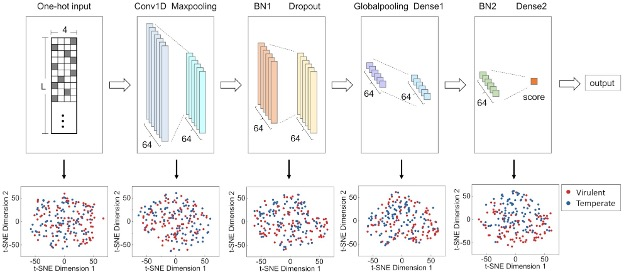
\includegraphics[width=1\linewidth]{figures/DeePhage_Model.jpg}
    \caption{Cấu trúc mạng nơ-ron học sâu và hình ảnh hóa 5 lớp bằng cách giảm kích thước của DeePhage}
    \label{fig:DeePhage_model}
\end{figure}

\subsection*{Kết quả thực nghiệm}

Dựa trên bảng kết quả kiểm thử chéo 5 lần, DeePhage vượt trộiso với PHACTS trên cả ba tiêu chí đánh giá Độ nhạy - Sensitivity, Độ đặc hiệu - Specificity và Độ chính xác- Accuracy ở tất cả các nhóm độ dài contig (từ 100–400 bp đến 1,200–1,800 bp).

Cụ thể:
\begin{itemize}
    \item Độ nhạy: DeePhage đạt từ 77.3\% đến 87.5\%, trong khi PHACTS chỉ đạt từ 64.7\% đến 73.7\%. 
    \item Độ đặc hiệu: DeePhage đạt từ 74.6\% đến 89.5\%, trong khi PHACTS chỉ đạt từ 26.3\% đến 42.3\%.
    \item Độ chính xác: DeePhage đạt độ chính xác cao từ 76.2\% đến 88.9\%, trong khi PHACTS dao động trong khoảng 48.6\% đến 54.8\%
\end{itemize}

Kết quả này cũng khẳng định ưu thế vượt trội của mô hình học sâu so với các mô hình học máy truyền thống trong việc giải quyết cùng nhiệm vụ phân loại thực khuẩn.

Ngoài ra, khi so sánh về hiệu năng, DeePhage xử lý 100 trình tự DNA chỉ mất 10s, nhanh hơn PHACTS 810 lần (135 phút)

\section{PhaTYP}

PhaTYP\cite{shang2023phatyp} là một mô hình học sâu thực hiện nhiệm vụ phân loại thực khuẩn thể trên dữ liệu metagenomics, tương tự như DeePhage. Tuy nhiên, thay vì sử dụng mạng nơ-ron tích chập (CNN) như DeePhage, PhaTYP áp dụng kiến trúc \textbf{BERT} (\textit{Bidirectional Encoder Representations from Transformers}). 

\subsection*{Chiến lược huấn luyện}

PhaTYP được huấn luyện qua hai nhiệm vụ: Học tự giám sát và Tinh chỉnh. 
\begin{itemize}
    \item \textbf{Nhiệm vụ học tự giám sát (Self-supervised learning)}: Mô hình học biểu diễn chuỗi DNA bằng cách dự đoán các đoạn bị che khuất tương tự như BERT trong xử lý ngôn ngữ tự nhiên.
    \item \textbf{Nhiệm vụ tinh chỉnh (Fine-tuning)}: Sau khi học biểu diễn DNA, mô hình được tinh chỉnh để phân loại thực khuẩn.
\end{itemize}
\begin{figure}[H]
    \centering
    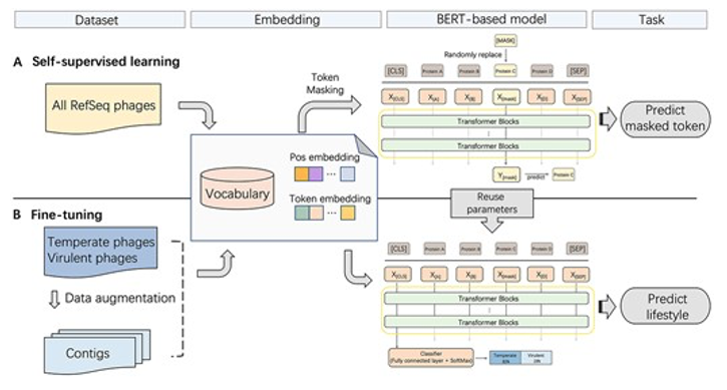
\includegraphics[width=1\linewidth]{figures/PhaTYP_Model.png}
    \caption{Kiến trúc mô hình PhaTYP sử dụng BERT}
    \label{fig:enter-label}
\end{figure}

\subsection*{Tập dữ liệu sử dụng}
\paragraph{Giai đoạn học tự giám sát:} dữ liệu được lấy từ cơ sở dữ liệu \textbf{NCBI RefSeq 2022}, bao gồm tổng cộng 3474 bộ gen của thực khuẩn. Mỗi bộ gen được cắt thành các đoạn có độ dài khác nhau: 5, 10, 15 và 20 kilobase pairs (kbp). Đối với mỗi bộ gen, 10 đoạn contig ngẫu nhiên được tạo ra, dẫn đến tổng cộng \textbf{142,434} đoạn contig được thu thập để phục vụ quá trình huấn luyện mô hình.

\paragraph{Giai đoạn phân loại:} dữ liệu được lấy từ cùng nguồn \textbf{NCBI RefSeq 2022} như ở giai đoạn học tự giám sát. Tập dữ liệu bao gồm 1290 thực khuẩn thể độc lực (\textit{virulent}) và 577 thực khuẩn thể ôn hoà (\textit{temperate}). Từ mỗi loại, 10.000 contig được tạo ngẫu nhiên với độ dài nằm trong khoảng từ 100 base pairs (bp) đến 20 kilobase pairs (kbp). Tổng cộng, tập dữ liệu huấn luyện cho giai đoạn này gồm \textbf{160,000 contig}, được xây dựng sao cho cân bằng giữa hai lớp.

\subsection*{Phương pháp và kỹ thuật chính}
PhaTYP sử dụng biểu diễn k-mer và kiến trúc BERT để học đặc trưng ngữ nghĩa của DNA, sau đó tinh chỉnh cho nhiệm vụ phân loại vòng đời thực khuẩn thể. 

Cụ thể:
\begin{itemize}
    \item Sử dụng biểu diễn DNA dưới dạng chuỗi k-mer làm đầu vào (tương tự token trong NLP).
    \item Áp dụng kiến trúc Transformer của BERT để học biểu diễn ngữ nghĩa của DNA.
    \item Tinh chỉnh lớp đầu ra cho nhiệm vụ phân loại thực khuẩn.
\end{itemize}

\subsection*{Kết quả thực nghiệm}

Dựa trên kết quả so sánh hiệu suất trên tập dữ liệu kiểm tra có mức độ tương đồng thấp, có thể nhận thấy rằng \textbf{PhaTYP vượt trội rõ rệt so với cả DeePhage và PHACTS} ở cả ba tiêu chí: độ nhạy (Sensitivity), độ đặc hiệu (Specificity) và độ chính xác (Accuracy).

\begin{table}[ht]
\centering
\caption{So sánh hiệu suất của PhaTYP với các công cụ khác.}
\label{tab:PhaTPY_Result}
\begin{tabular}{|l|c|c|c|}
\hline
\textbf{Công cụ} & \textbf{Sensitivity} & \textbf{Specificity} & \textbf{Accuracy} \\
\hline
PhaTYP             & \textbf{0.99} & \textbf{0.89} & \textbf{0.94} \\
PhaTYP (without SSL)   & 0.98 & 0.86 & 0.92 \\
DeePhage           & 0.96 & 0.86 & 0.91 \\
BACPHLIP           & 0.98 & 0.84 & 0.90 \\
PHACTS             & 0.90 & 0.69 & 0.74 \\
PhagePred          & 0.57 & 0.83 & 0.67 \\
\hline
\end{tabular}
\end{table}

So với DeePhage, PhaTYP đạt độ nhạy cao hơn (0.99 so với 0.96), độ đặc hiệu cao hơn (0.89 so với 0.86), và tổng độ chính xác cũng cao hơn (0.94 so với 0.91). Mặc dù mức chênh lệch không quá lớn, kết quả này cho thấy việc áp dụng học tự giám sát (\textit{Self-Supervised Learning – SSL}) và kiến trúc BERT đã giúp PhaTYP học được các đặc trưng ngữ nghĩa hiệu quả hơn từ dữ liệu DNA, đặc biệt trong các mẫu khó và ít tương đồng.

So với PHACTS là công cụ sử dụng mô hình học máy truyền thống, PhaTYP tạo ra kết quả khác biệt lớn. PHACTS chỉ đạt 0.90 về độ nhạy, 0.69 về độ đặc hiệu và 0.74 về độ chính xác – thấp hơn nhiều so với PhaTYP ở mọi chỉ số. 

Những điều này cho thấy khả năng vượt trội của các mô hình học sâu khi thực hiện phân loại trên dữ liệu metagenomics. Từ đó, PhaTYP khẳng định khả năng ứng dụng hiệu quả trong thực tế với nhiệm vụ phân loại thực khuẩn.

\section{DeepPL}
Tương tự PhaTYP, DeepPL\cite{zhang2024deeppl} là một mô hình phân loại vòng đời thực khuẩn thể được phát triển dựa trên kiến trúc \textbf{DNABERT} – phiên bản thích ứng của BERT cho dữ liệu chuỗi DNA. Điểm khác biệt của DeepPL là tập trung khai thác thông tin từ các đoạn gen liên quan đến chu kì tiềm tan, vốn chỉ có ở phage ôn hoà, nhằm cải thiện độ chính xác trong phân loại.

\subsection*{Dữ liệu sử dụng}

\textbf{Tập huấn luyện}:
\begin{itemize}
    \item 1262 bộ gen thực khuẩn thể độc lực
    \item 557 bộ gen thực khuẩn thể ôn hoà
\end{itemize}
    
\textbf{Tập kiểm thử}:
\begin{itemize}
    \item 245 bộ gen thực khuẩn thể độc lực
    \item 129 bộ gen thực khuẩn thể ôn hoà
\end{itemize}
    
\textbf{Tiền xử lí dữ liệu:}
Do chỉ có các thực khuẩn thể ôn hòa mới có các gen kích hoạt/duy trình chu kỳ tiềm tan, nhóm tác giả thực hiện trích xuất những đoạn gen có chức năng này. Tiếp theo, thực hiện thao tác chuẩn hoá dữ liệu:
\begin{itemize}
    \item Loại bỏ các đoạn gen nếu có nhiều hơn 10 ký tự không thuộc loại \texttt{A, T, G, C}.
    \item Với các đoạn có không quá 10 ký tự không hợp lệ, thay thế ngẫu nhiên thành A, T, G hoặc C.
\end{itemize}


\subsection*{Chiến lược tạo mẫu}
Mục tiêu của giai đoạn này, nhóm tác giả muốn tạo mẫu cân bằng giữa hai nhãn. Trong khi đặc điểm của các mẫu gen của thực khuẩn thể ôn hoà thường rất ngắn, còn mẫu gen của thực khẩn thể độc lực thường dài hơn. Do đó, nhóm tác giả dùng kĩ thuật cửa sổ trượt với kích thước cửa sổ là 100bp nhưng với các bước trượt khác nhau:
\begin{itemize}
    \item Với mẫu gen của thực khuẩn thể ôn hoà: bước trượt chỉ 1 bp để tạo ra nhiều mẫu hơn.
    \item Với mẫu gen của thực khuẩn thể ôn hoà: bước trượt 91 bp để tạo ra số mẫu tương đương.
\end{itemize}
Kết quả thu được 547{,}810 chuỗi từ gen thực khuẩn thể độc lực và 500{,}765 chuỗi từ gen thực khuẩn thể ôn hoà. Gần đạt được tỉ lệ cân bằng (50:50) đối với hai nhãn.

\subsection*{Phương pháp và kiến trúc mô hình}

\begin{itemize}
    \item \textbf{Tiền xử lý}: Chuỗi DNA được chia thành các đoạn \textit{6-mer}, tạo thành chuỗi tương tự văn bản.
    \item \textbf{Biểu diễn}: Sử dụng mô hình huấn luyện trước DNABERT để ánh xạ các 6-mer sang không gian vector.
    \item \textbf{Tinh chỉnh}: Tinh chỉnh DNABERT trên tập dữ liệu đã gán nhãn để thực hiện phân loại thực khuẩn.
\end{itemize}
\begin{figure}[H]
    \centering
    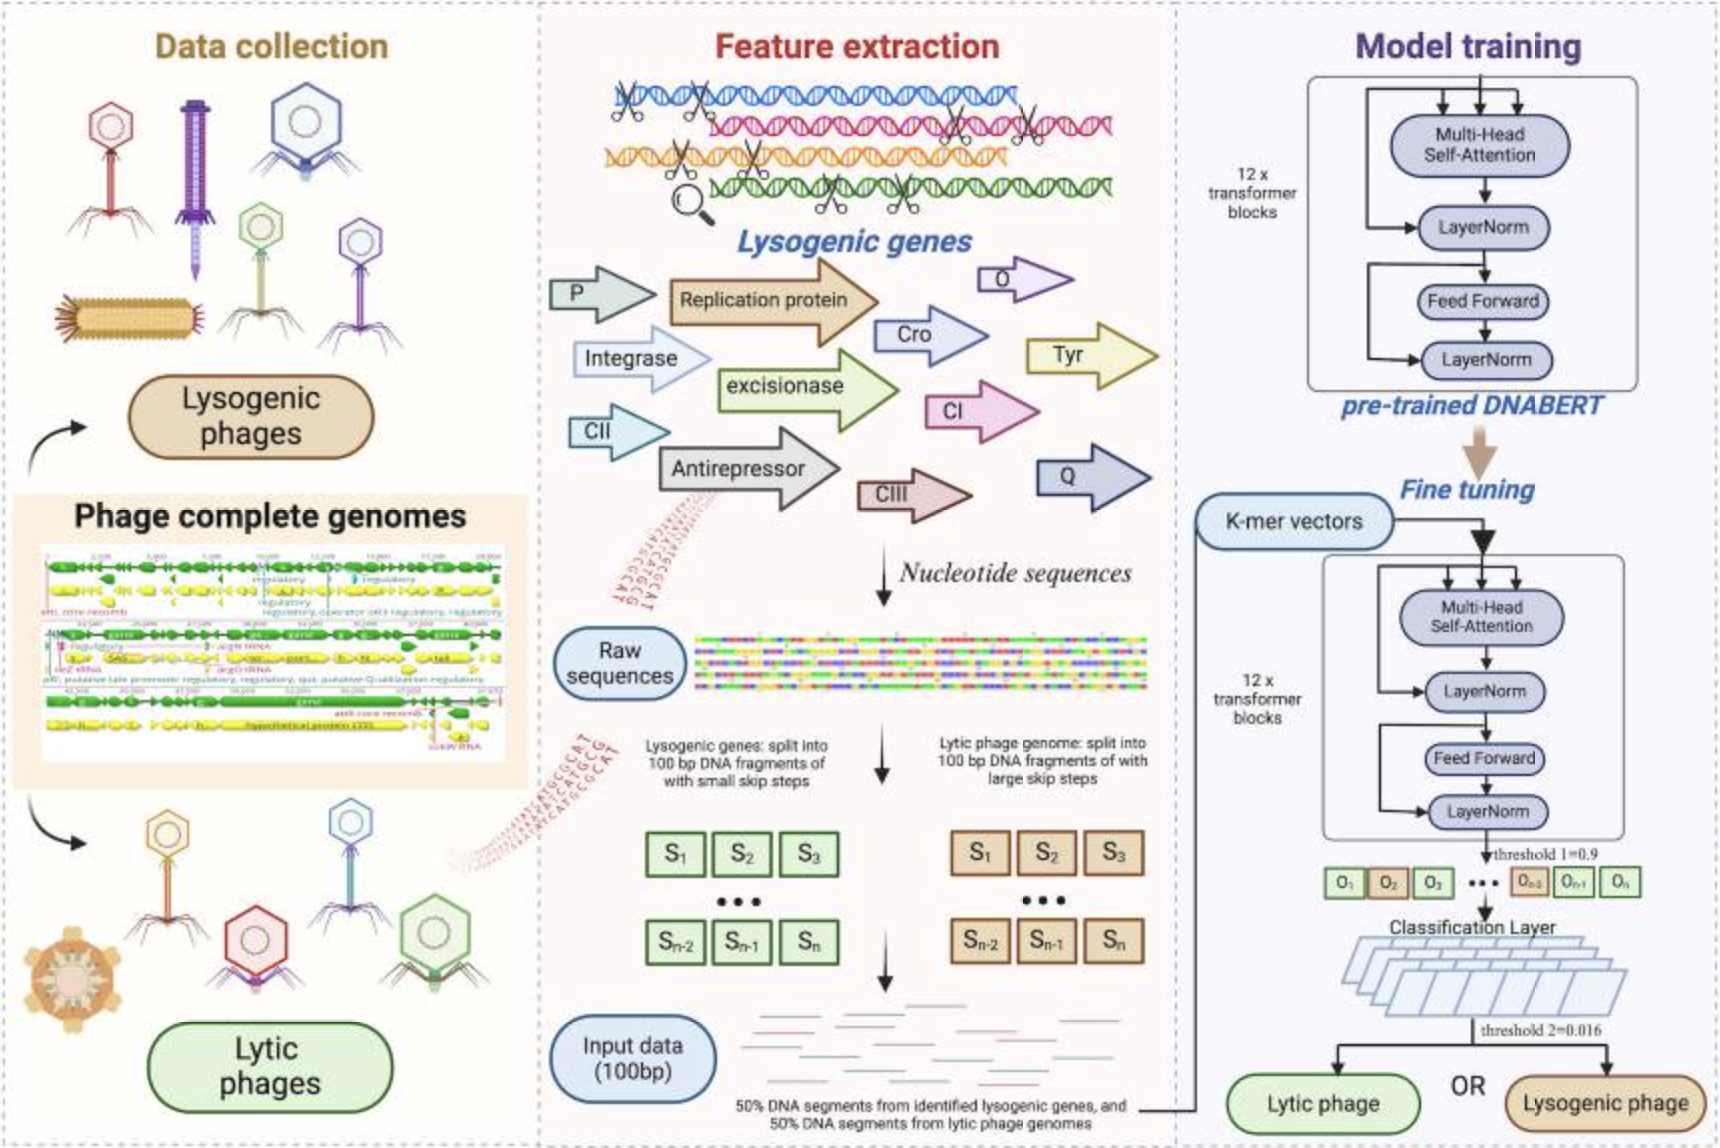
\includegraphics[width=1\linewidth]{figures/DeepPL_model.png}
    \caption{Kiến trúc mô hình DeepPL sử dụng NDABERT}
    \label{fig:DeepPL_model}
\end{figure}

\subsection*{Kết quả thực nghiệm}

\begin{table}[ht]
\centering
\caption{So sánh hiệu suất giữa DeepPL và các công cụ khác.}
\label{tab:performance_comparison_deeppl}
\begin{tabular}{|l|c|c|c|c|c|}
\hline
\textbf{Công cụ} & \textbf{Sensitivity} & \textbf{Specificity} & \textbf{Accuracy} & \textbf{F1-score} & \textbf{MCC} \\
\hline
DeepPL   & \textbf{92.24}  & 95.91 & 94.65 & 0.92 & 0.53 \\
PhaTYP   & 90.44 & 97.47 & \textbf{94.91} & 0.92 & 0.53 \\
DeePhage & 78.61 & \textbf{98.13} & 89.83 & 0.86 & 0.49 \\
PHACTS   & 38.94 & 79.77 & 48.66 & 0.53 & 0.14 \\
PhageAI  & 83.33 & 96.08 & 91.17 & 0.87 & 0.50 \\
\hline
\end{tabular}
\label{tbl:deeppl}
\end{table}

\textbf{DeepPL} cho thấy hiệu suất cao và ổn định trong bài toán phân loại thực khuẩn, với độ nhạy 92.24\%, độ đặc hiệu 95.91\%, độ chính xác 94.65\%, F-score đạt 0.92 và hệ số tương quan Matthews (MCC) là 0.53.

So với PhaTYP, DeepPL không tạo được sự khác biệt lớn. DeepPL đạt độ nhạy cao hơn (92.24\% so với 90.44\%). Nhưng so sánh độ chính xác tổng thể, DeepPL (94.65\%) thấp hơn so với PhaTYP (94.91\%).